\section{Ergebnisse}
Es werden mehrere Laufzeitmessungen durchgeführt, um die Auswrikung der Parallelisierung zu erfassen. Zur Vergleichbarkeit und Minimierung von Einflüssen durch sich ändernde Lasten der virtuellen Maschinen in der Cloud werden alle Messungen sequentiell vorgenommen. Zur Aufwandsbegrenzung wird eine Stichprobengröße von $n = 10$ Messungen pro Messklasse gewählt. Für eine statistisch fundierte Aussage notwendig wäre ein höhere Anzahl an Messungen. Die Messklassen werden über die Anzahl der verwendeten Rechenknoten festgelegt. Messungen werden mit einem bis sieben Rechenknoten durchgeführt. Gemessen wird zuerst die benötigte Laufzeit, eine gleichbleibende Datei bestehend aus einer Zahl der Größenordnung von $400.000$ Wörtern zu sortieren. Anschließend wird mit einer Datei von doppelter Wörterzahl die Messreihe wiederholt.
\\
Eine Messergebnis ist die mithilfe der Standard Template Bibliothek std::chrono gemessene Zeit, welche im Programmablauf des Master-Knotens zwischen dem Zeitpunkt unmittelbar vor der Verteilung der Teilelemente 
des zu sortierenden Textes an die Slave-Knoten und dem Zeitpunkt unmittelbar nach dem Zusammenführen der Ergebnisse der Slave-Rechenknoten verstreicht.
Das arithmetische Mittel sowie die Standardabweichung der Messungen mit kürzerer Wörterzahl sind in der oberen Hälfte von Tabelle 1 aufgeführt. Die entsprechenden Werte zur größeren Datei sind in der unteren Hälfte von Tabelle 1 dargestellt.
\\
Bei der Messung mit kleiner Datei und genau einem Rechenknoten ist eine im Vergleich zu anderen Rechenknotenanzahlen erhöhte Unsicherheit zu erkennen. Die mittlere benötigte Rechenzeit ist signifikant höher als bei anderen Messungen mit einer Rechenknotenanzahl größer eins. Bei den Rechenknotenanzahlen vier, fünf und sechs ist eine im Vergleich geringe Abweichung festzustellen.
\\
Die Mittelwerte der Zeiten für die kleinere Datei liegen ab einer Rechenknotenanzahl von 4 eng beieinander. Mit den vorliegenden Daten kann keine statistisch begründete Aussage getroffen werden, ob sich die Rechenzeit ab einer Knotenzahl von 4 noch messbar verändert. Der scheinbar deutlich niedrigere Mittelwert der 7. Messung wird durch eine höhere Messunsicherheit relativiert.
\\
Dies kann auch im Kastenschaubild (Whisker Plot) zu den Messungen der kleineren Datei, Abbildung 2, nachvollzogen werden.


%\section{Auswertung}
Grundsätzlich versprechen sich die Autoren von ideal implementierter Parallelisierung einen messbaren Zusammenhang von der Anzahl der verwendeten Rechenknoten und der resultierenden Laufzeit.
\\
Auch hier ist die vermutete, anfängliche und deutliche 
Absenkung der Laufzeiten über die Anzahl der Rechenknoten zu erkennen. Ebenfalls fällt ein starker Ausreißer bei der Knotenzahl eins auf. Auch bei Knotenzahlen zwei, vier und sechs 
gibt es solche Ausreißer. Bei den Knotenzahlen vier und sechs, welche eine relativ geringe Standardabweichung aufweisen, ebenfalls Ausreißer nach oben. 
Im Kontext der niedrigen Standardabweichung bedeutet das einerseits, dass die restlichen Messwerte dieser Messreihen besonders konsistent sind. Andererseits kann dies ein Hinweis darauf sein, dass die gemessenen Zeiten durch Zufall besonders konsistent und niedrig ausgefallen sind.

\begin{table*}
	\caption{Zeitmessungen mit kleiner und großer Wörterzahl}
	\label{zeiten_tabelle_lang_und_kurz}
	\begin{tabularx}{\textwidth}{@{}l*{10}{C}c@{}}
		\toprule
		Anzahl der Rechenknoten & 1 & 2 & 3 & 4 & 5 & 6 & 7 \\ 
		\midrule
		$\bar{t}_{wenige Wörter}$ $\mathrm{[ms]}$ & 4382.9 & 2413.7 & 2148.5 & 1728.6 & 1715.9 & 1621.6 & 1574.6 \\
		$\sigma_{wenige Wörter}$ $\mathrm{[ms]}$ & 491.2 & 128.0 & 113.9 & 72.2 & 70.9 & 62.3 & 112.4 \\
		\addlinespace
		$\bar{t}_{viele Wörter}$ $\mathrm{[ms]}$ & 13114.2 & 8857.0 & 6643.7 & 5913.3 & 5072.5 & 4727.8 & 4855.2 \\
		$\sigma_{viele Wörter}$ $\mathrm{[ms]}$ & 99.3 & 240.1 & 202.2 & 261.0 & 125.1 & 105.0 & 180.1 \\
		\bottomrule
	\end{tabularx}
\end{table*}

\begin{figure}[!t]
    \centering
    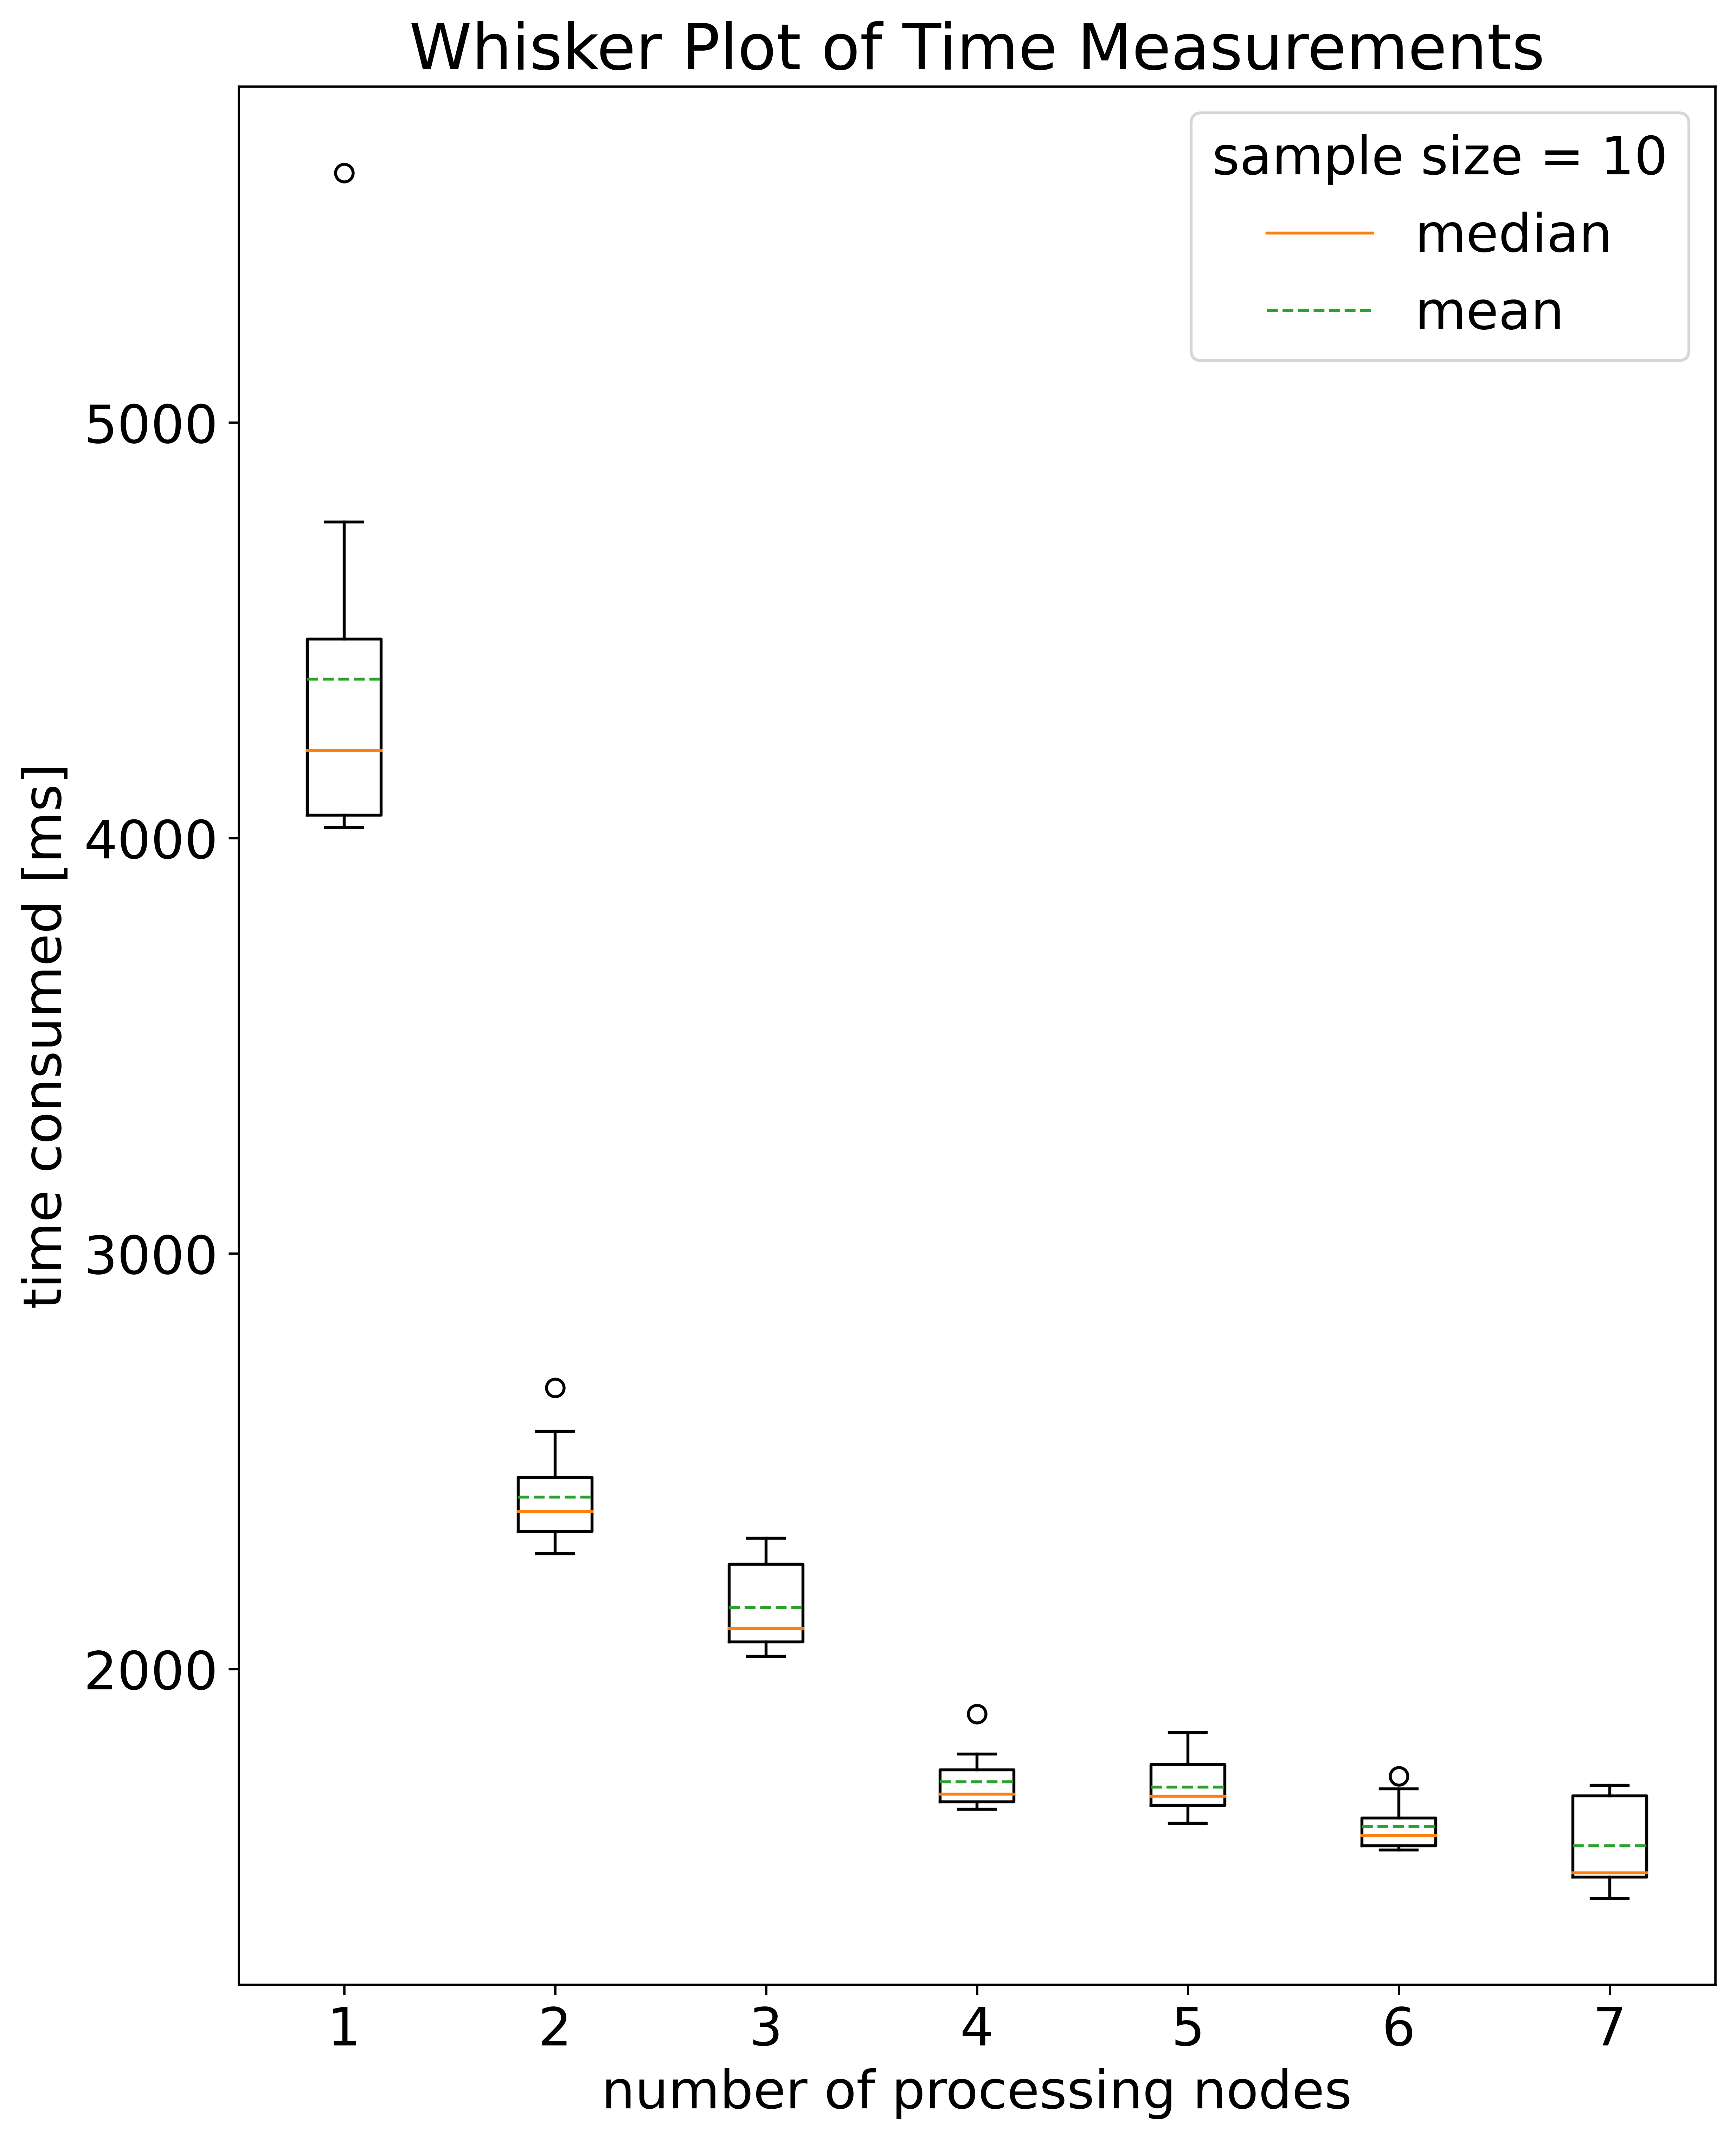
\includegraphics[width=3.5in]{boxplots.png}
    \caption{Messwerte zur kleineren der beiden getesteten Dateien dargestellt in einem Kastenschaubild}
    \label{boxplot_times}
\end{figure}

So lassen die beobachteten Phänomene insgesamt darauf schließen, dass die Parallelisierung in ihrer für das Projekt durchgeführten Implementierung eine signifikante Absenkung der Laufzeit von bis zu einer Größenordnung von 60\% mit sich bringt. Dieser Effekt ist jedoch stark begrenzt und flacht mit einer steigenden Rechenknotenanzahl schnell ab bzw. verschwindet gänzlich. Die Effizienz pro Rechenknoten nimmt damit bei steigender Anzahl von Rechenknoten schnell ab.
Für genauere Aussagen ist eine größere Anzahl an Messungen pro Messklasse für nötig.
\\
Eine Deutung für die Beobachteten Ergebnisse: die Rechenknoten in der Cloud sind mittels Ethernet miteinander verbunden, was das Senden und Empfangen von Nachrichten erstens nicht zeitlich deterministisch und zweitens anfällig für unregelmäßige und längere Laufzeiten macht. Offenbar bewegt sich bei der betrachteten Dateigröße das Senden und Empfangen von Nachrichten an mehr Knoten ab einer Knotenzahl von ca. vier in einer ähnlichen Größenordnungen wie der Laufzeitgewinn, welcher dadurch entsteht, dass ein Rechenknoten nur eine geringere Anzahl an Arbeit (Wörter sortieren) hat. Die Autoren vermuten, dass bei einer deutlich größeren Datei (mit mehr Wörtern), ein Laufzeitgewinn auch bei größeren Knotenzahlen zu messen sein wird.
\\
Um diese These zu untersuchen, wurden die Messungen mit einer Datei der doppelten Wörterzahl wiederholt. Die Ergebnisse sind in der unteren Hälfte von Tabelle 1 und in Abbildung 3 zu begutachten. Wieder ist ein zunächst signifikanter Abfall der Rechenzeiten zu beobachten bevor auch hier der oben beschriebene Effekt der Abflachung auftritt. War es oben der Schritt von Knotenzahl 3 auf 4, welcher eine letzte messbare Reduzierung der Laufzeit mit sich brachte, ist es nun der Schritt von Knotenzahl 4 auf 5. Dies widerlegt die Antithese, dass mehr Rechenaufwand sich \textit{nicht} auf den Auftretenszeitpunkt dieses Effektes auswirkt.
\\
Jedoch ist insbesondere unter Betrachtung der absoluten Laufzeitwerte festzustellen, dass eine größerer Arbeitsaufwand nicht ohne weiteres durch mehr Rechenknoten kompensierbar scheint. Während bei der kleineren Datei die Laufzeiten sich im Bereich von $1.6\mathrm{s}$ eingependelt haben, werden bei doppelter Wörteranzahl etwa $5\mathrm{s}$ benötigt. Der zugrunde liegende Merge Sort Algorithmus ist Teil der Komplexitätsklasse ${\mathcal{O}(n\log{n})}$. Es ist damit zu erwarten, dass die Laufzeiten bei gleicher Knotenzahl sich mehr als verdoppeln, also überlinear steigen. Dies ist in Tabelle 1 zu erkennen. Bei gleicher Knotenzahl benötigt die Datei mit doppelter Länge durchweg mehr als die doppelte Laufzeit. Allerdings haben die Autoren in Anbetracht der gewählten Aufteilungsstrategie erwartet, dass mit mehr Knoten die größere Wörteranzahl zu großen Teilen kompensiert wird. Ein Vergleich der Mittelwerte in Tabelle 1 wiederlegt diese These deutlich. Die Anzahl der Wörter, welche jeder Knoten im Fall \glqq kleine Datei, 3 Rechenknoten\grqq{} und im Fall \glqq große Datei, 6 Rechenknoten\grqq{} zu sortieren hat, ist identisch. Die benötigten mittleren Zeiten, $~2\mathrm{s}$ vs. $~6\mathrm{s}$ widerlegen diese Erwartung deutlich. Die Autoren vermuten die Funktion \textit{merge\_back()} als primäre und den erhöhten Sende- und Empfangsaufwand als sekundäre Erklärung hierfür. Grund hierfür ist, dass die Funktion \textit{merge\_back()} allein auf dem Master Knoten läuft. Entsprechend werden hier die Vorteile der Parallelisierung nicht mehr genutzt. Bei genauerer Betrachtung von \textit{merge\_back()} ist zudem zu erkennen, dass die Laufzeit der Funktion stark von der Größe der zu sortierenden, vorsortierten Einzelelemente abhängt. Bei doppelter Wörterzahl sind doppelt so viele vorsortierte Wörtergruppen zu sortieren. Daher wäre aus Sicht der Autoren eine Erweiterung Funktion \textit{merge\_back()} um eine Parallelisierungsstrategie der erste Angriffspunkt, um das Programm für große Wörterzahlen weiter zu optimieren.\\
\begin{figure}[!t]
	\centering
	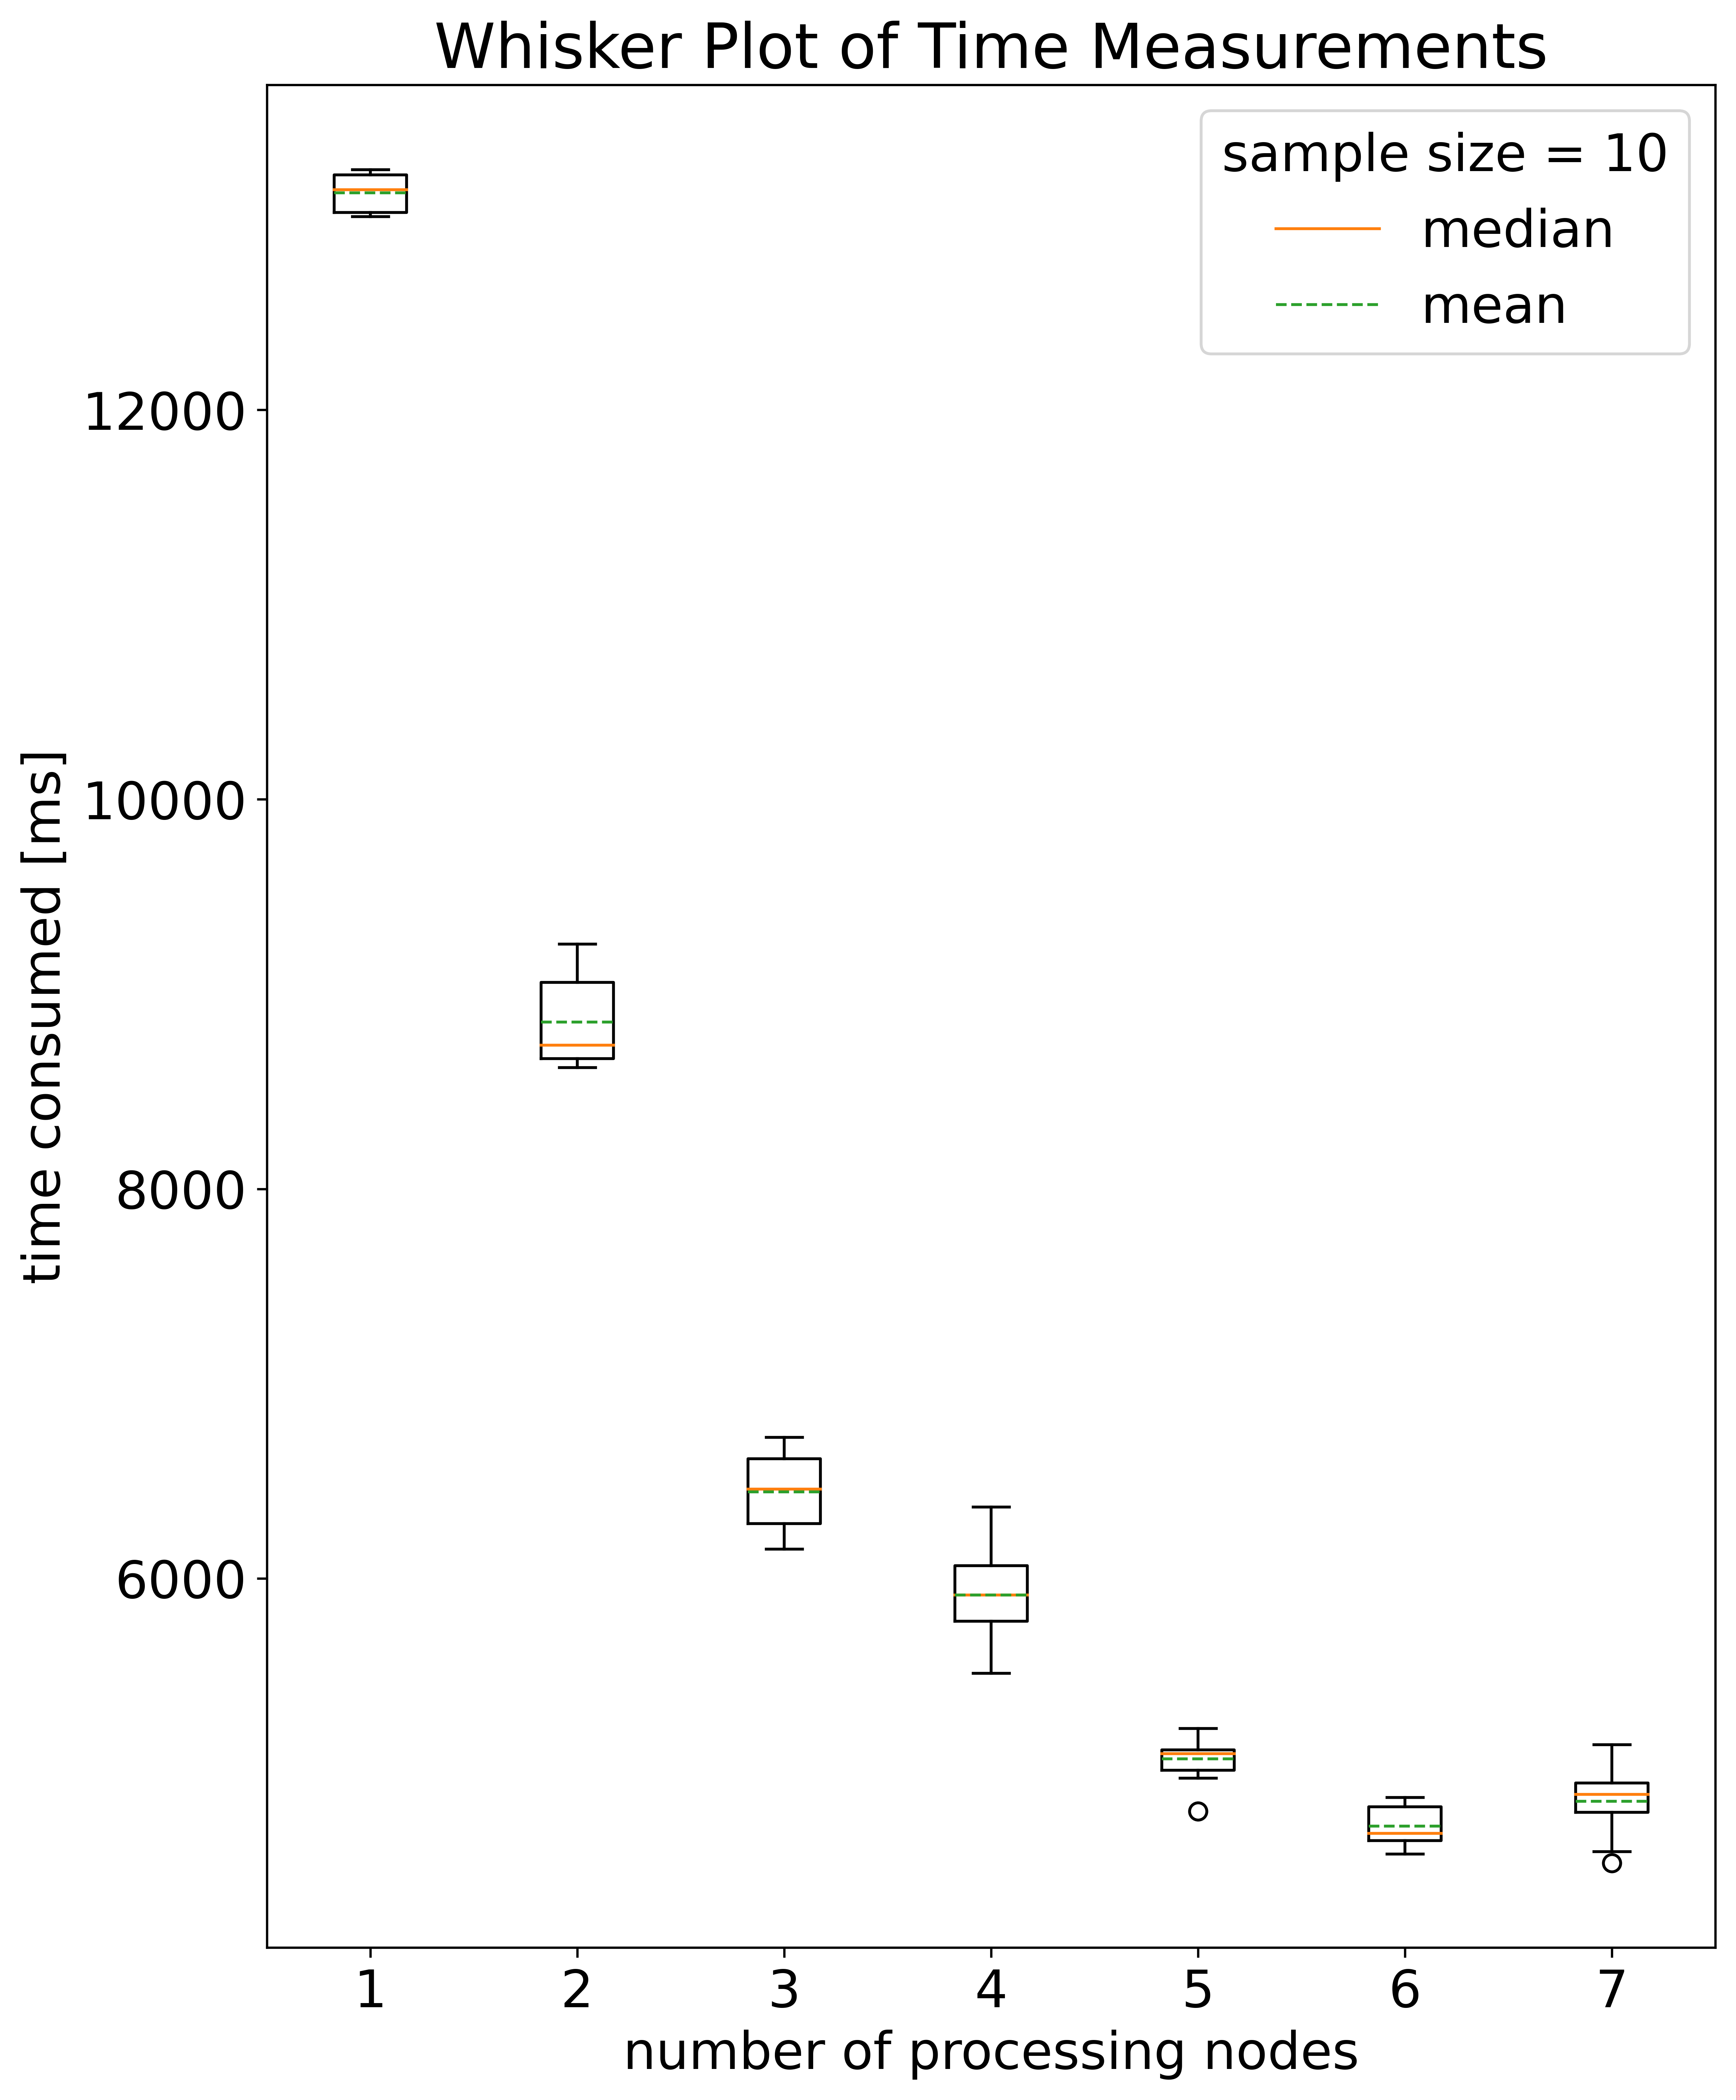
\includegraphics[width=3.5in]{boxplots_long.png}
	\caption{Messwerte zur größeren der beiden getesteten Dateien dargestellt in einem Kastenschaubild}
	\label{boxplot_times_long}
\end{figure}